\documentclass{article}
\usepackage{graphicx} % Required for inserting images
\usepackage[utf8]{vietnam}
\usepackage{titlesec}
\usepackage{titling}
\usepackage{amsmath}
\usepackage{natbib}
\usepackage[a4paper, top=2.5cm, bottom=2.5cm, left=3cm, right=3cm]{geometry}
\usepackage{lipsum} 
\usepackage{enumitem}
\usepackage{subfiles}
\usepackage{wrapfig}
\usepackage{graphicx}
\usepackage{float}
\usepackage{booktabs} % For table formatting
\usepackage{array} % For better alignment
\usepackage[hidelinks]{hyperref} 
\usepackage{longtable}
\usepackage{geometry}
\usepackage{etoolbox}
\usepackage{xcolor}
\usepackage{longtable}
\usepackage{colortbl}
\usepackage{cleveref}
\usepackage{amsfonts}
\usepackage{tocloft}
\setlength{\cftsecnumwidth}{4em} % Bạn có thể điều chỉnh giá trị 2.5em cho phù hợp
\geometry{margin=1in}

\renewcommand\thesection{\Roman{section}}
% \setmainfont{Times New Roman}
% Thiết lập kích thước chữ 13pt
\renewcommand{\normalsize}{\fontsize{12pt}{15.6pt}\selectfont}
\renewcommand\thesection{\Roman{section}}  % Để \section hiển thị chữ số La Mã (I, II, ...)
\renewcommand\thesubsection{\arabic{subsection}}  % Để \subsection chỉ hiển thị số (1, 2, 3, ...)
%\renewcommand\thesubsubsection{\arabic{subsection}.\arabic{subsubsection}}  % Để \subsubsection hiển thị 1.1, 1.2, ...
\newcommand{\bigsection}[1]{%
  \refstepcounter{bigsection}%
  \section*{Phần \Alph{bigsection}: #1}%
  \addcontentsline{toc}{section}{Phần \Alph{bigsection}: #1}
}

\newcounter{bigsection}
\begin{document}

\pagenumbering{gobble}
\begin{titlepage}
\begin{figure}[!t]
\centering
\Large{TRƯỜNG ĐẠI HỌC SÀI GÒN \\ KHOA CÔNG NGHỆ THÔNG TIN
}\\[0.4in]


\includegraphics[width = 4in]{images/SGU.png}
% \caption*{}
\end{figure}

\centering
\LARGE{\textbf{Báo cáo môn: Ngôn ngữ lập trình C\#}}\\[0.2in]
\LARGE{\textbf{Đề tài: Quản lý thư quán}}\\[0.4in]
\LARGE{\textbf{Giảng viên hướng dẫn: Nguyễn Minh Cảnh}}\\[0.4in]

\LARGE{Sinh viên thực hiện}\\[0.2in]
\LARGE{\textbf{Quách Hữu Vinh - 3122410477}}\\[0.1in]
\LARGE{\textbf{Thới Thanh Vương - 3122410487}}\\[0.1in]
\LARGE{\textbf{Nguyễn Trần Uyển Nhi - 3122410281}}\\[0.1in]
\LARGE{\textbf{Bùi Lê Duy Thái - 3122410377}}\\[0.1in]
\LARGE{\textbf{Phạm Công Thành - 3122310386}}\\[0.1in]
\LARGE{\textbf{Kiều Tấn Tài - 3123410314}}\\[0.1in]

% \large{Supervisor: XXXXX}\\
% \large{Co-supervisor: XXXXX}\\[0.5in]

\vfill
\begin{center}
    \Large{Tháng 05 - 2025}
\end{center}
% \small{nhichan276@gmail.com}
\newpage
\end{titlepage}.
\clearpage 

\pagenumbering{arabic}
\tableofcontents

\newpage
\bigsection{Tổng quan về ứng dụng và đặc tả yêu cầu}
\section{Giới thiệu}
Ngày nay, khi công nghệ phát triển mạnh mẽ, nhu cầu quản lý tài nguyên, đặc biệt là sách và thiết bị trong thư quán, đang trở thành một thách thức lớn đối với các thư quán, trường học, và các tổ chức giáo dục. Việc theo dõi số lượng sách, tài liệu, thiết bị mượn/trả, và tính toán phí phạt cho các tài nguyên quá hạn là vấn đề quan trọng mà thư quán cần giải quyết một cách hiệu quả.
\\ \\
Đề tài "Quản lý thư quán" ra đời nhằm cung cấp một giải pháp toàn diện, giúp thư quán quản lý sách và thiết bị dễ dàng hơn. Hệ thống giúp theo dõi các thông tin như tên sách, tác giả, thể loại, số lượng tồn kho, tình trạng mượn/trả, và phí mượn, từ đó giúp nhân viên quản lý thư quán không chỉ tiết kiệm thời gian mà còn nâng cao hiệu quả công việc. Hệ thống còn hỗ trợ việc tính toán các khoản phí quá hạn và cung cấp các báo cáo thống kê chi tiết, giúp thư quán dễ dàng quản lý và đưa ra các quyết định hợp lý.
\\ \\
Hệ thống được phát triển với kiến trúc OOP (Object-Oriented Programming) trong ứng dụng WinForm C\# và được triển khai trên nền tảng ASP.NET cho phần web. Kiến trúc này giúp xây dựng các lớp đối tượng rõ ràng, dễ bảo trì và mở rộng trong tương lai. Cơ sở dữ liệu sử dụng MySQL kết hợp với giao diện người dùng trên WinForm cho các tác vụ quản lý trong thư quán và ASP.NET cho các tính năng web giúp người dùng truy cập từ xa. Việc sử dụng cả hai nền tảng này sẽ mang lại sự linh hoạt, đồng thời giúp thư quán quản lý hiệu quả các tài nguyên sách và thiết bị. Giải pháp này không chỉ tiết kiệm thời gian cho nhân viên mà còn tạo ra một dịch vụ tiện ích, hỗ trợ công việc học tập và nghiên cứu cho tất cả người dùng, đồng thời nâng cao trải nghiệm người dùng trên cả nền tảng desktop và web.

\section{Đặt tả yêu cầu}
\subsection{Chức năng của phần mềm}
\subsubsection{Chức năng của Winform}
\begin{table}[H]
\centering
\renewcommand{\arraystretch}{1.6}
\begin{tabular}{|p{4.5cm}|p{10cm}|}
\hline
\textbf{Quản Lý Sản Phẩm} & 
- Thêm, sửa, xóa thông tin sách và thiết bị \newline
- Nhập/xuất dữ liệu dưới dạng Excel \newline
- Tra cứu sách/thiết bị \newline
- Cập nhật trạng thái sách/thiết bị \\
\hline
\textbf{Quản Lý Giao Dịch} & 
- Cập nhật thông tin mượn/trả sách và thiết bị: mã sách, mã thiết bị, mã người dùng, ngày mượn, hạn trả \newline
- Kiểm tra tình trạng sách và thiết bị trước khi mượn \newline
- Ghi nhận thông tin đặt trước sách và thiết bị \newline
- Ghi nhận thông tin trả sách và thiết bị, cập nhật trạng thái sách \newline
- Cảnh báo sách và thiết bị quá hạn và gửi thông tin qua email \\
\hline
\textbf{Quản Lý Thành Viên} & 
- Tra cứu người dùng theo mã, tên, số điện thoại \newline
- Xóa thông tin người dùng khi không còn hoạt động \newline
- Admin có quyền thêm/sửa/xóa tài khoản nhân viên \newline
- Nhân viên thư quán có quyền thao tác với sách, thiết bị và mượn/trả \newline
- Quản lý số lượng thành viên ra vào thư quán \\
\hline
\textbf{Quản Lý Vi Phạm và Quy Định} & 
- Ghi nhận vi phạm của người dùng, lý do vi phạm, phạt tiền nếu có \newline
- Thêm/sửa/xóa những quy định \newline
- Quản lý danh sách quy định, cập nhật mức phạt theo từng lỗi \newline
- Theo dõi trạng thái thanh toán vi phạm \\
\hline
\textbf{Báo cáo và thống kê} & 
- Thống kê số lượng sách, thiết bị hiện có, sách/thiết bị đã mượn/quá hạn \newline
- Báo cáo danh sách thành viên hoạt động (mượn/trả) nhiều nhất \newline
- Báo cáo danh sách thành viên ra vào thư quán \\
\hline
\end{tabular}
\end{table}

\subsubsection{Chức năng của Website}
\begin{table}[H]
\centering
\renewcommand{\arraystretch}{1.6}
\begin{tabular}{|p{5cm}|p{10cm}|}
\hline
\textbf{Đăng Nhập/Đăng Ký Thành Viên} & 
- Đăng ký thành viên mới \newline
- Đăng nhập tài khoản bằng user account/email \newline
- Hỗ trợ lấy lại mật khẩu của tài khoản thành viên \newline
- Xem/Cập nhật thông tin thành viên \\
\hline
\textbf{Đặt Trước Sản Phẩm} & 
- Cho phép thành viên đặt trước sách/thiết bị có sẵn trong kho để đảm bảo có thể mượn khi có sẵn. \newline
- Cung cấp thông tin về các sách/thiết bị đã đặt trước, tình trạng của sách và thời gian kỳ kiến có thể mượn. \newline
- Thành viên sẽ nhận thông báo khi sách/thiết bị có thể mượn. \\
\hline
\textbf{Xem Lịch Sử Giao Dịch Của Thành Viên} & 
- Thành viên có thể xem lại các sách đã mượn trước đó, bao gồm ngày mượn, ngày trả, và tình trạng của sách. \newline
- Thành viên sẽ nhận nhắc nhở về việc trả sách, cũng như các sách đang được mượn và chưa trả. \\
\hline
\textbf{Đánh Giá và Phản Hồi} & 
- Hiển thị các sách chưa được trả đúng hạn và thông báo về việc phạt hoặc gia hạn sách. \newline
- Thành viên có thể đánh giá và viết nhận xét về sản phẩm. \newline
- Quản lý phản hồi của khách hàng, giải đáp thắc mắc. \\
\hline
\textbf{Cảnh Báo Vi Phạm} & 
- Cảnh báo thành viên về các hành vi vi phạm như quá hạn trả sách/thiết bị, làm hỏng sách/thiết bị, hoặc vi phạm các quy định khác của thư quán. \newline
- Hiển thị thông báo khi thành viên bị phạt hoặc có sách/thiết bị bị mất/méo mó do vi phạm quy định. \newline
- Cung cấp lịch sử các lần vi phạm của thành viên, bao gồm các lỗi vi phạm, mức độ vi phạm, mức phạt, và ngày xử lý vi phạm. \newline
- Cảnh báo người dùng nếu có quá nhiều lần vi phạm và có thể khóa tài khoản tạm thời hoặc vĩnh viễn. \newline
- Người dùng sẽ nhận thông báo khi tài khoản bị khóa và có thể yêu cầu mở khóa sau khi thành thạo các điều kiện (nộp phạt, cam kết không tái phạm). \newline
- Cho phép người dùng yêu cầu gia hạn nếu có lý do hợp lý cho việc trả sách trễ hạn. \\
\hline
\end{tabular}
\end{table}

\newpage
\bigsection{Thiết kế dự án}
\section{Giao diện}

\subsection{Winform}
\begin{figure} [H]
    \centering
    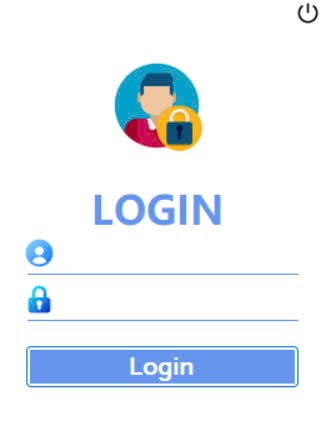
\includegraphics[width=0.3\linewidth]{images//Winform/login.png}
    \caption{Login winform}
    \label{fig:enter-label}
\end{figure}

\begin{figure} [H]
    \centering
    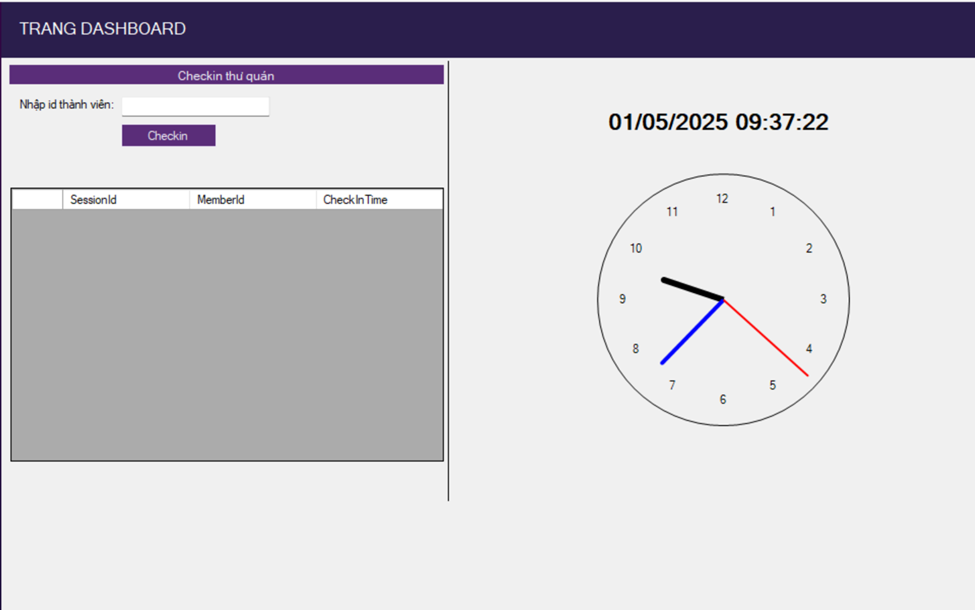
\includegraphics[width=1\linewidth]{images//Winform/dashboard.png}
    \caption{Trang Dashboard}
    \label{fig:enter-label}
\end{figure}

\begin{figure} [H]
    \centering
    \includegraphics[width=1\linewidth]{images//Winform/page chính.png}
    \caption{Trang Dashboard}
    \label{fig:enter-label}
\end{figure}

\begin{figure} [H]
    \centering
    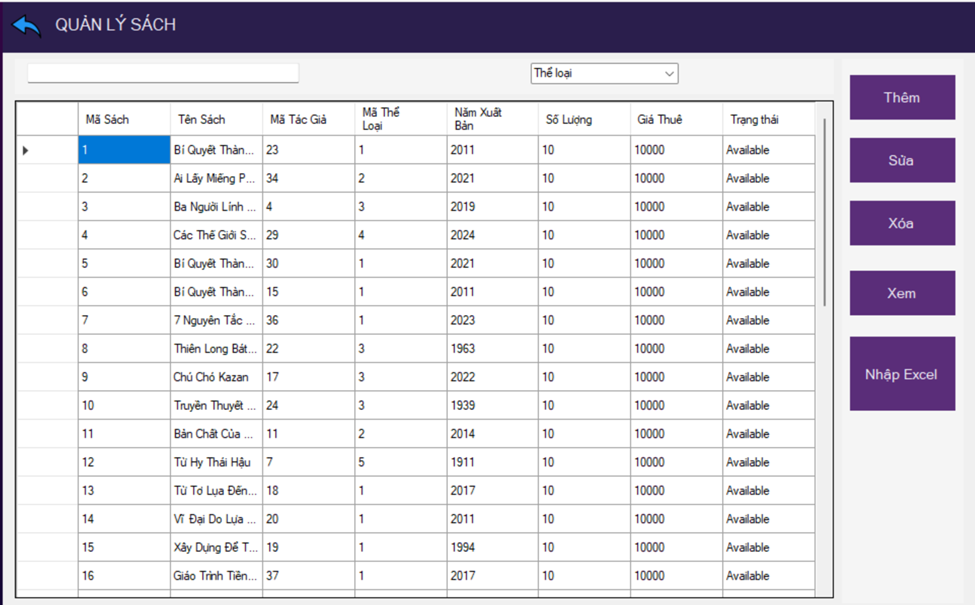
\includegraphics[width=1\linewidth]{images//Winform/page quản lý.png}
    \caption{Trang quản lý sách}
    \label{fig:enter-label}
\end{figure}

\begin{figure} [H]
    \centering
    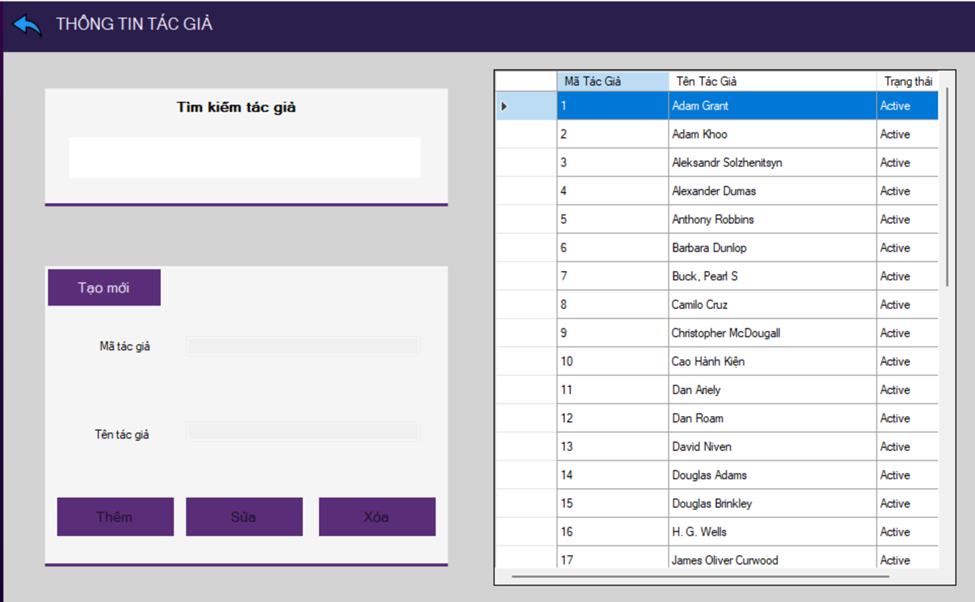
\includegraphics[width=1\linewidth]{images/Winform/page tác giả.png}
    \caption{Trang quản lý tác giả}
    \label{fig:enter-label}
\end{figure}

\begin{figure} [H]
    \centering
    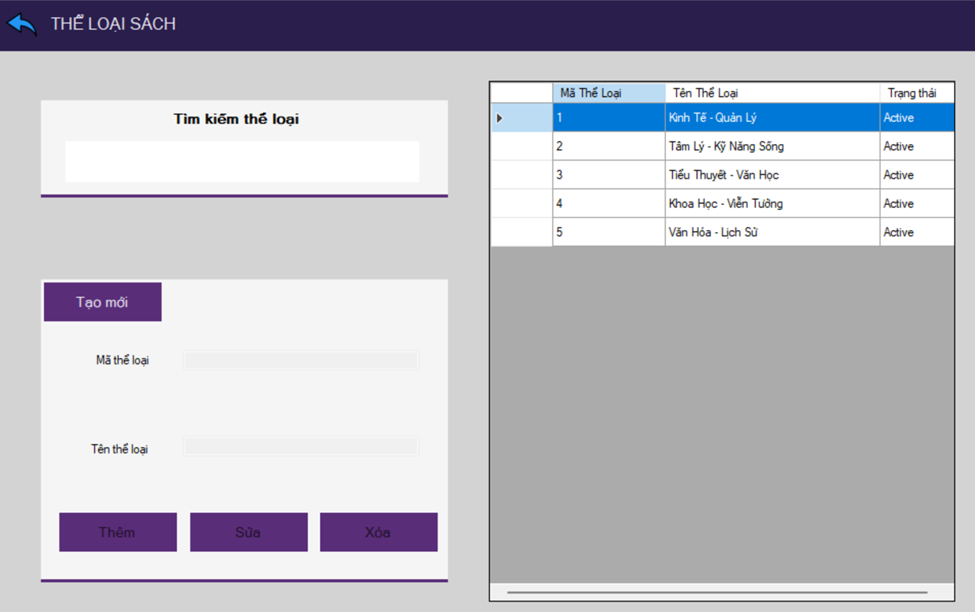
\includegraphics[width=1\linewidth]{images//Winform/page thể loại.png}
    \caption{Trang quản lý thể loại sách}
    \label{fig:enter-label}
\end{figure}

\begin{figure} [H]
    \centering
    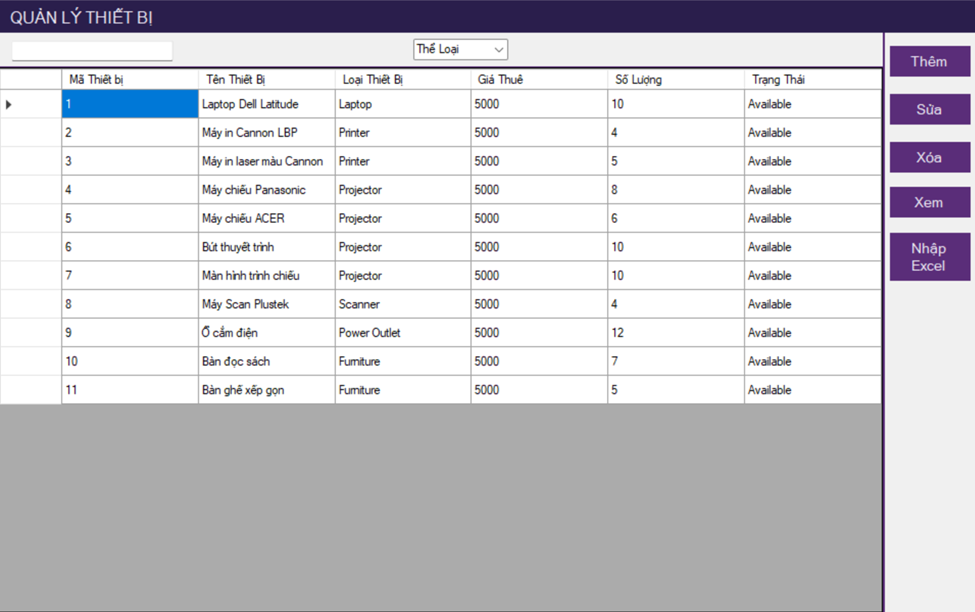
\includegraphics[width=1\linewidth]{images//Winform/page thiết bị.png}
    \caption{Trang quản lý thiết bị}
    \label{fig:enter-label}
\end{figure}

\begin{figure} [H]
    \centering
    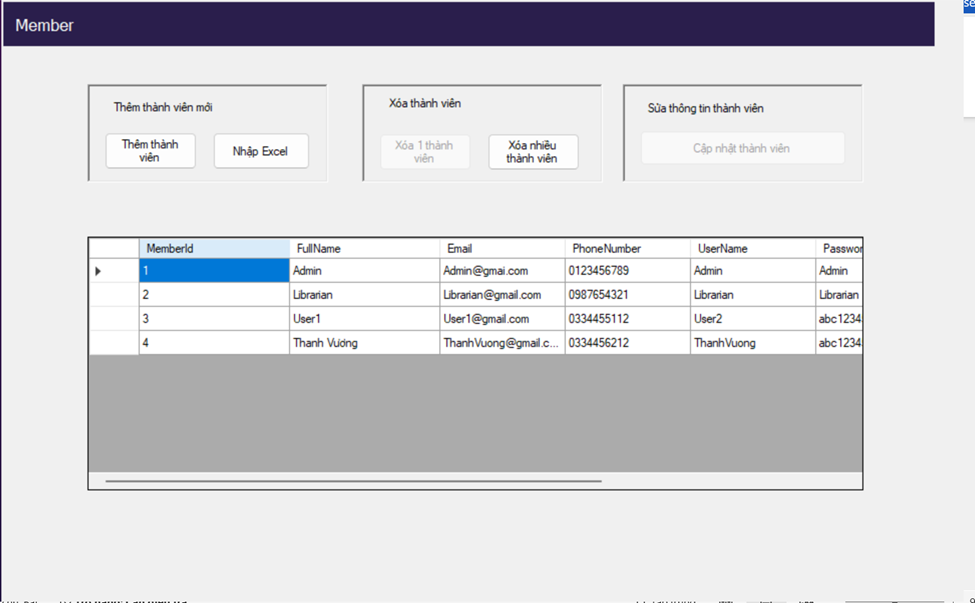
\includegraphics[width=1\linewidth]{images//Winform/page thành viên.png}
    \caption{Trang quản lý thành viên}
    \label{fig:enter-label}
\end{figure}

\begin{figure} [H]
    \centering
    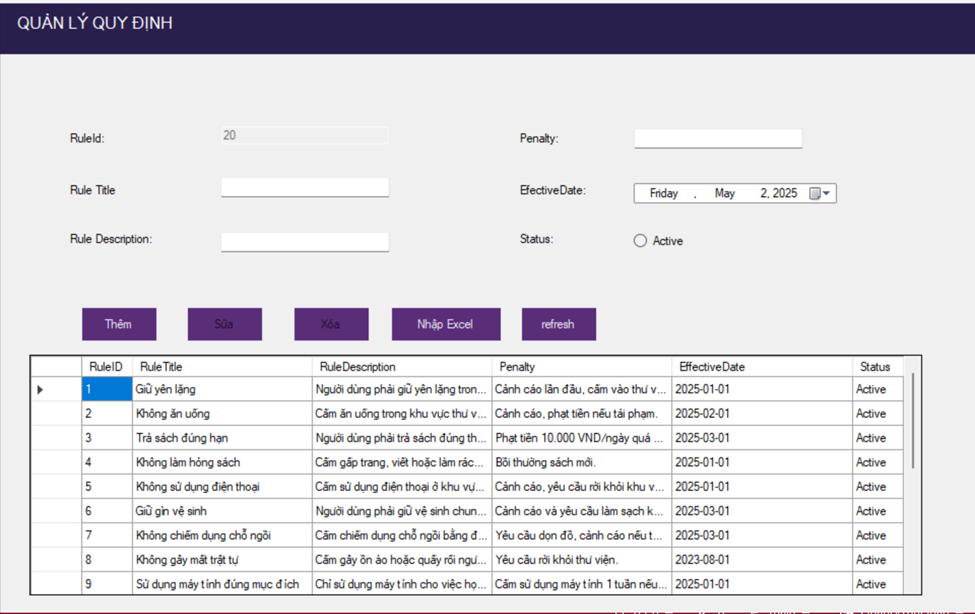
\includegraphics[width=1\linewidth]{images/Winform/page quy định.png}
    \caption{Trang quản lý quy định}
    \label{fig:enter-label}
\end{figure}

\begin{figure} [H]
    \centering
    \includegraphics[width=1\linewidth]{images//Winform/page giao dịch.png}
    \caption{Trang quản lý giao dịch}
    \label{fig:enter-label}
\end{figure}

\begin{figure} [H]
    \centering
    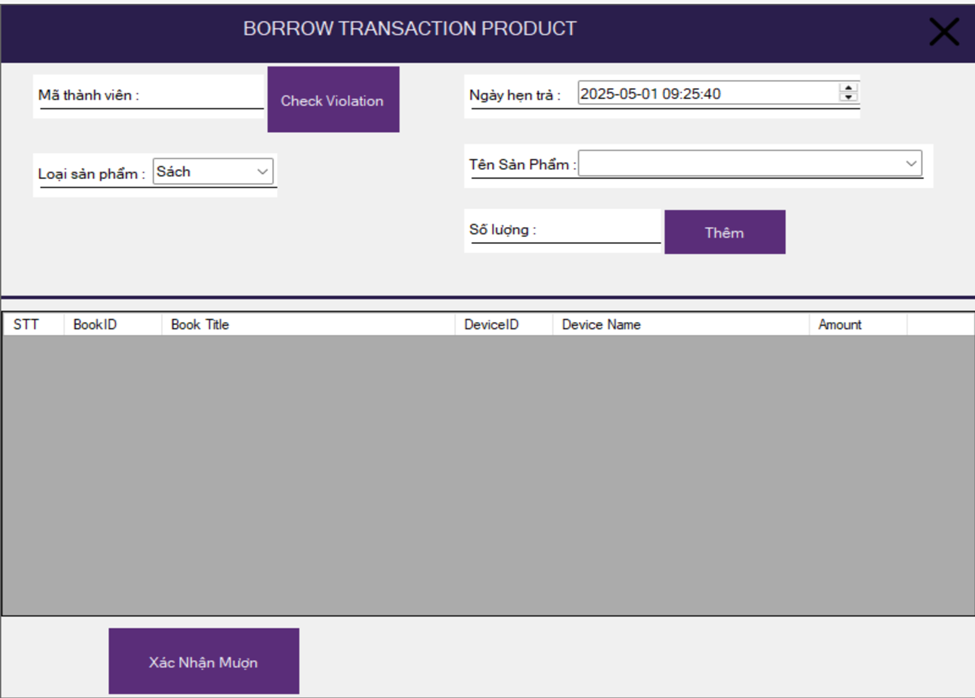
\includegraphics[width=1\linewidth]{images/Winform/page đk giao dịch.png}
    \caption{Trang đăng ký giao dịch}
    \label{fig:enter-label}
\end{figure}

\begin{figure} [H]
    \centering
    \includegraphics[width=1\linewidth]{images//Winform/page in4 giao dịch.png}
    \caption{Trang thông tin chi tiết giao dịch}
    \label{fig:enter-label}
\end{figure}

\begin{figure} [H]
    \centering
    \includegraphics[width=1\linewidth]{images//Winform/page vi phạm.png}
    \caption{Trang quản lý vi phạm}
    \label{fig:enter-label}
\end{figure}

\begin{figure} [H]
    \centering
    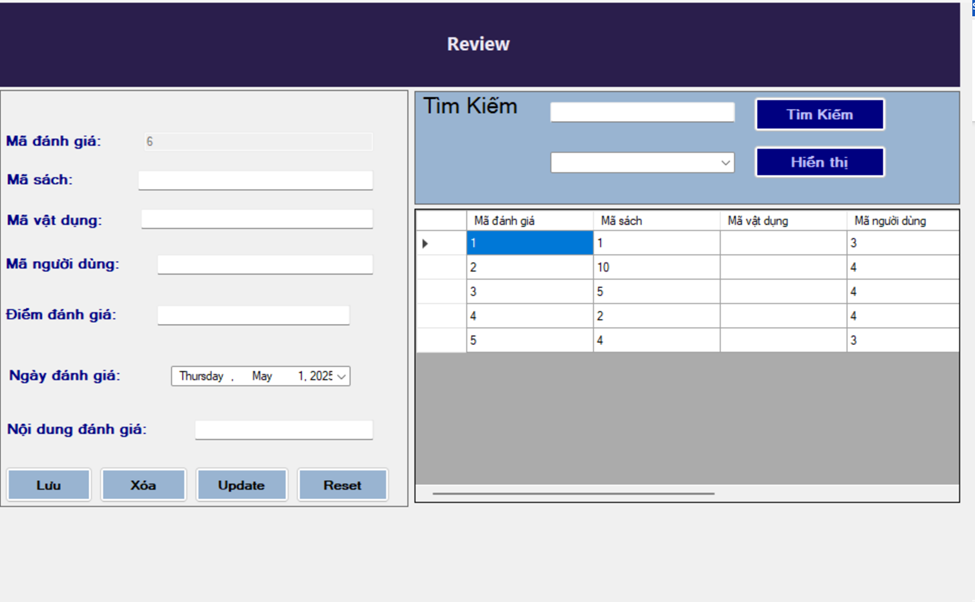
\includegraphics[width=1\linewidth]{images//Winform/page review.png}
    \caption{Trang Review}
    \label{fig:enter-label}
\end{figure}

\begin{figure}
    \centering
    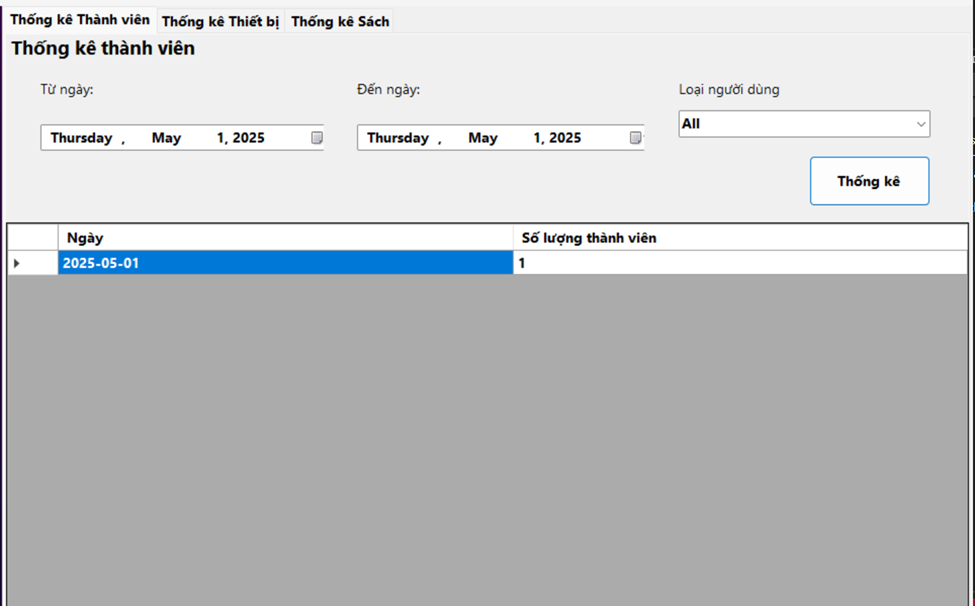
\includegraphics[width=1\linewidth]{images//Winform/page thống kê tv.png}
    \caption{Trang thống kê thành viên}
    \label{fig:enter-label}
\end{figure}

\begin{figure} [H]
    \centering
    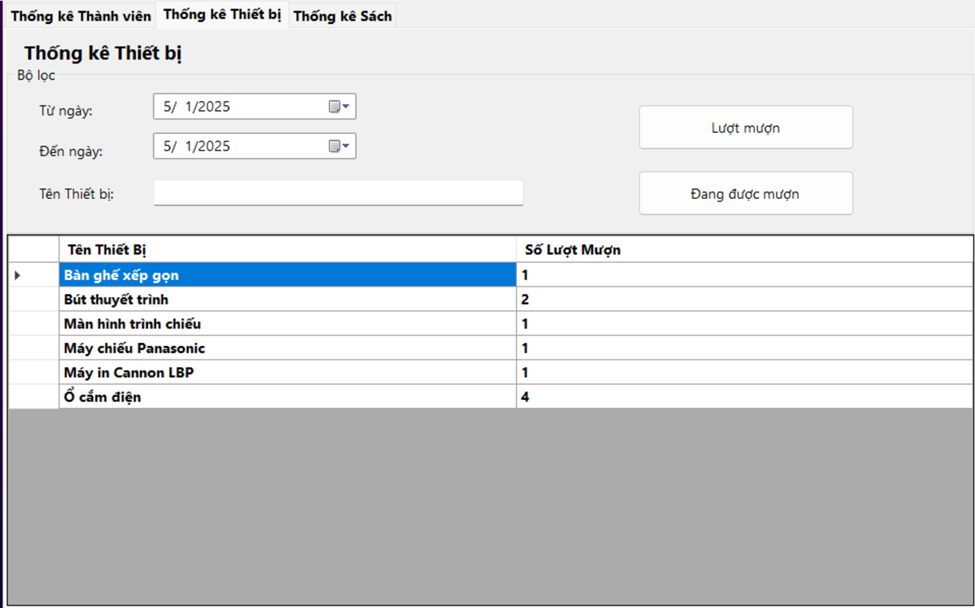
\includegraphics[width=1\linewidth]{images//Winform/page thống kê tb.png}
    \caption{Trang thống kê thiết bị}
    \label{fig:enter-label}
\end{figure}

\begin{figure} [H]
    \centering
    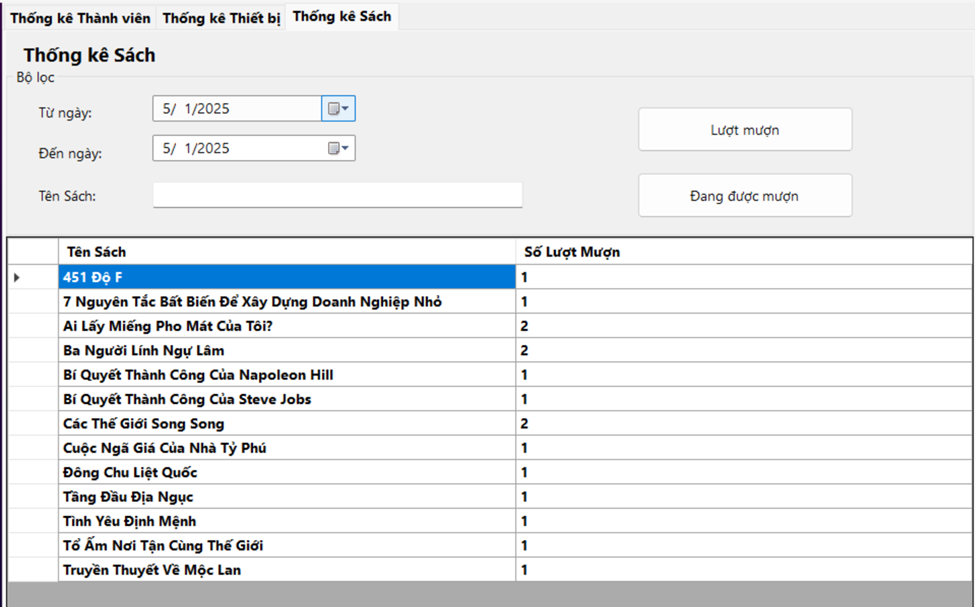
\includegraphics[width=1\linewidth]{images//Winform/page thống kê sách.png}
    \caption{Trang thống kê sách}
    \label{fig:enter-label}
\end{figure}

\subsection{Website}
\begin{figure} [H]
    \centering
    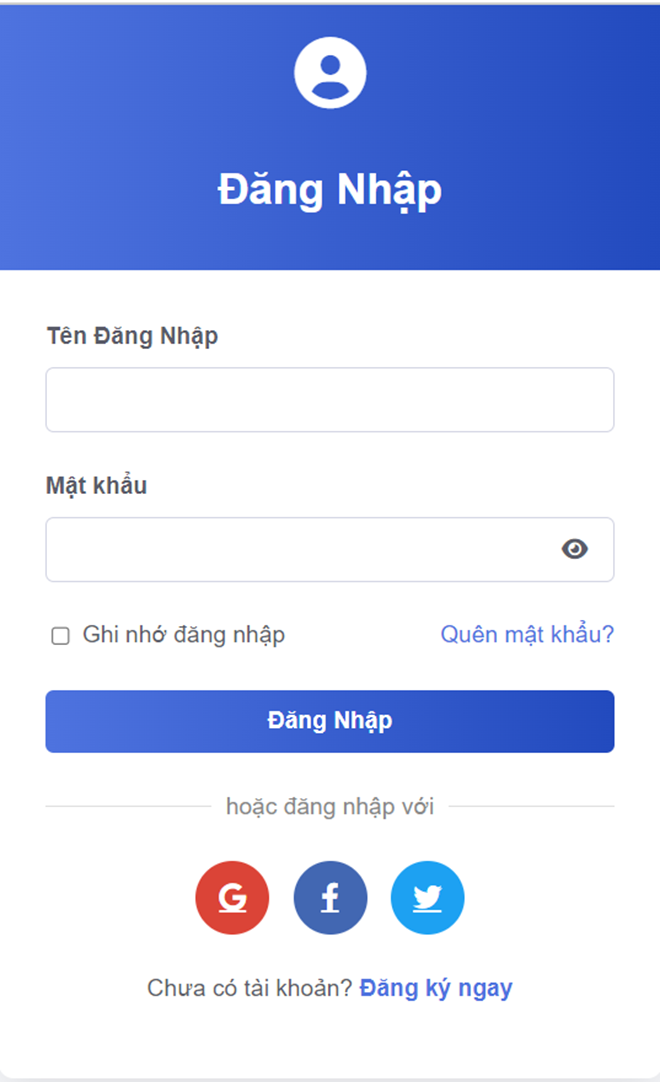
\includegraphics[width=0.3\linewidth]{images//Website/login.png}
    \caption{Login website}
    \label{fig:enter-label}
\end{figure}

\begin{figure} [H]
    \centering
    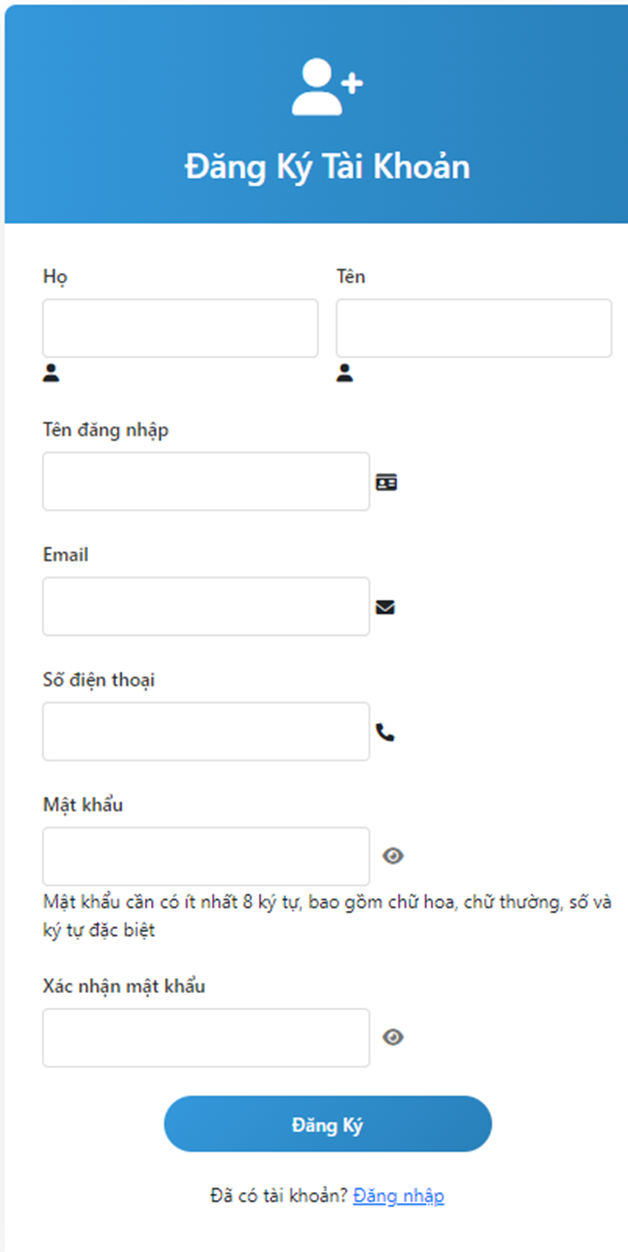
\includegraphics[width=0.3\linewidth]{images//Website/page đăng ký.png}
    \caption{Trang đăng ký}
    \label{fig:enter-label}
\end{figure}

\begin{figure} [H]
    \centering
    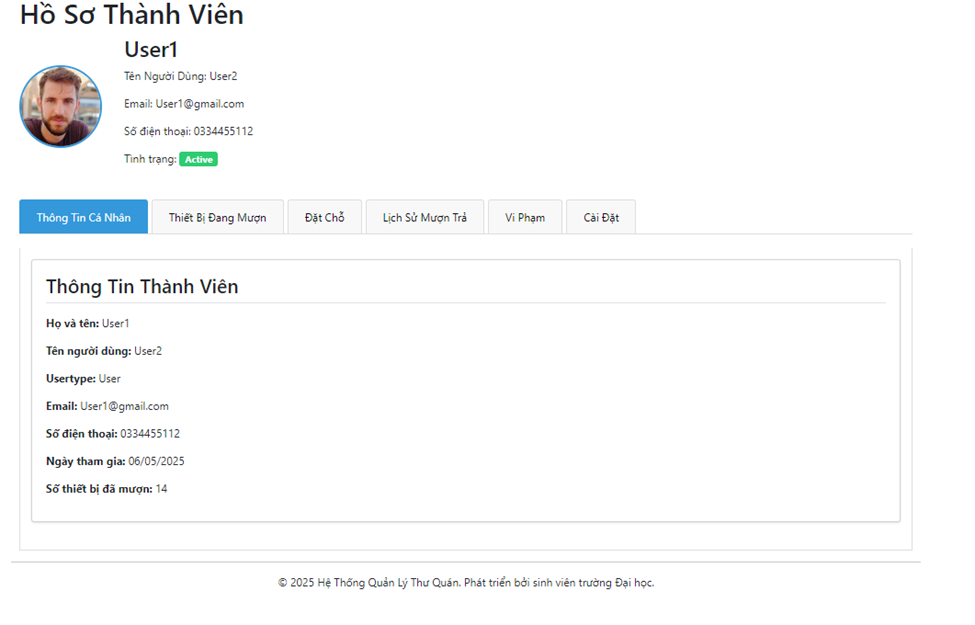
\includegraphics[width=1\linewidth]{images//Website/in4 tv.png}
    \caption{Trang thông tin cá nhân}
    \label{fig:enter-label}
\end{figure}

\begin{figure} [H]
    \centering
    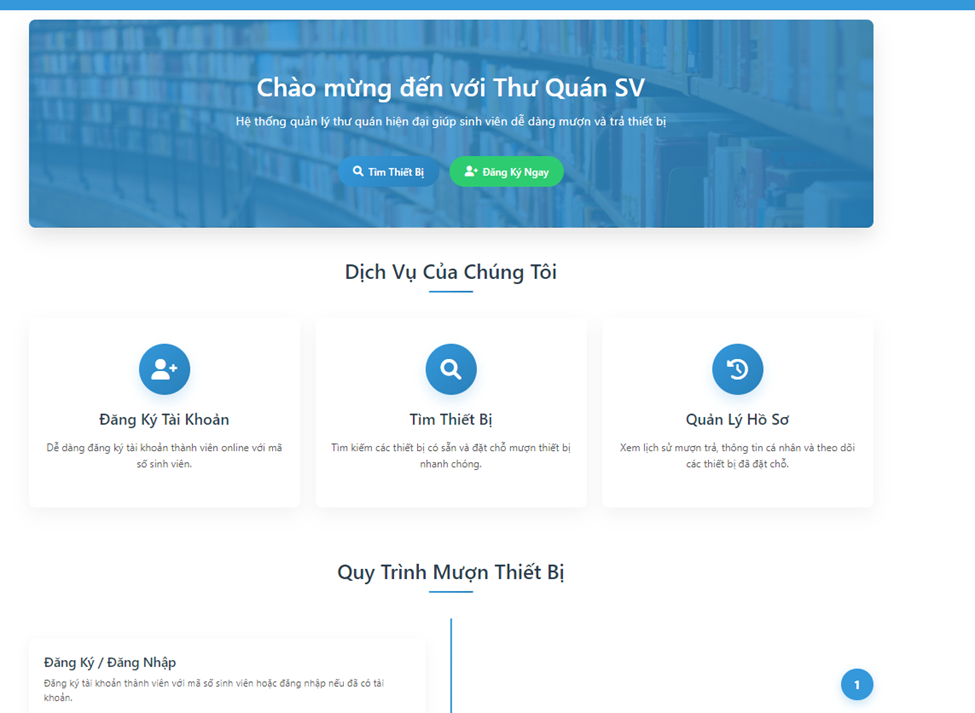
\includegraphics[width=0.9\linewidth]{images//Website/website.png}
    \caption{Trang chủ website}
    \label{fig:enter-label}
\end{figure}

\begin{figure} [H]
    \centering
    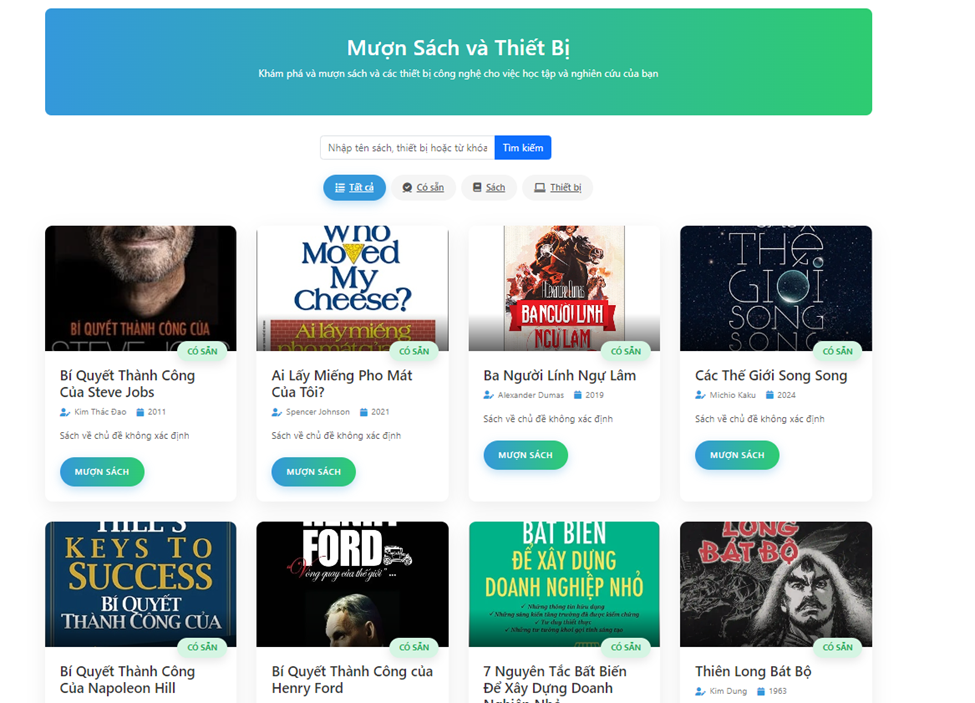
\includegraphics[width=0.9\linewidth]{images//Website/page đặt trước sp.png}
    \caption{Trang đặt trước sản phẩm}
    \label{fig:enter-label}
\end{figure}

\subsection{Cơ sở dữ liệu}
\subsubsection{ERD}
\begin{figure} [H]
    \centering
    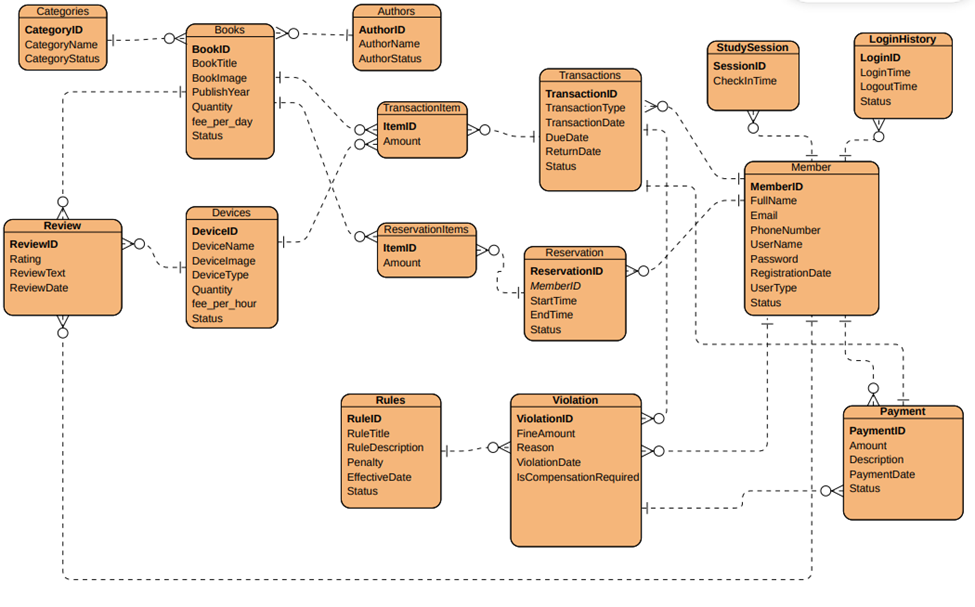
\includegraphics[width=1\linewidth]{images//CSDL/ERD.png}
    \label{fig:enter-label}
\end{figure}

\subsubsection{Mức logic}
\begin{figure} [H]
    \centering
    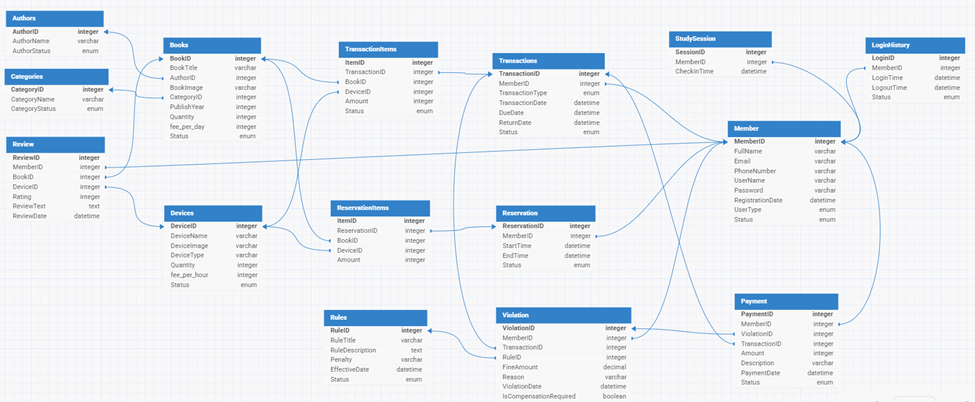
\includegraphics[width=1\linewidth]{images//CSDL/logic.png}
    \label{fig:enter-label}
\end{figure}


\newpage
\bigsection{Báo cáo kết quả}
\section{Winform}
\subsection{Chức năng đăng nhập hệ thống}
\begin{itemize}
    \item Cho phép người dùng nhập tên đăng nhập và mật khẩu để vào hệ thống với vai trò nhân viên hoặc quản trị viên.
    \item Kiểm tra thông tin đăng nhập và hiển thị cảnh báo khi sai.
\end{itemize}

\begin{figure} [H]
    \centering
    \includegraphics[width=0.3\linewidth]{images//Winform/login lỗi.png}
    \caption{Thông báo lỗi đăng nhập khi nhập sai}
    \label{fig:enter-label}
\end{figure}

\subsection{Chức năng quản lý sách}
Cho phép thêm, sửa, xóa thông tin sách, tra cứu theo tên sách hoặc thể loại, cập nhật trạng thái và quản lý hình ảnh bìa sách. Hỗ trợ nhập danh sách sách dưới dạng Excel.

\subsubsection{Quá trình thực thi thêm sách mới}
Bước 1: Nhấp chuột vào nút quản lý sách
\begin{figure} [H]
    \centering
    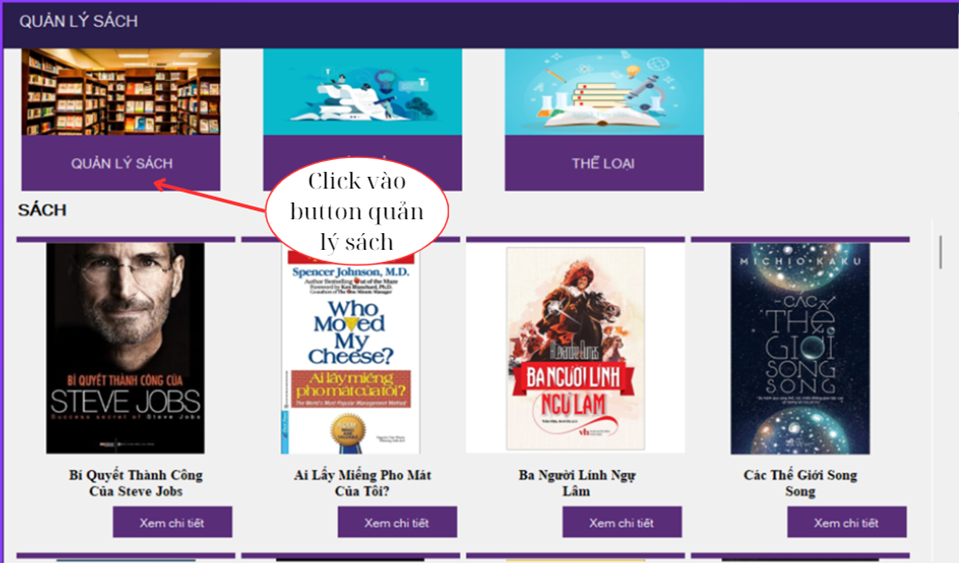
\includegraphics[width=0.8\linewidth]{images//Winform/thêm1.png}
    \label{fig:enter-label}
\end{figure}

Bước 2: Nhấp chuột vào nút thêm
\begin{figure} [H]
    \centering
    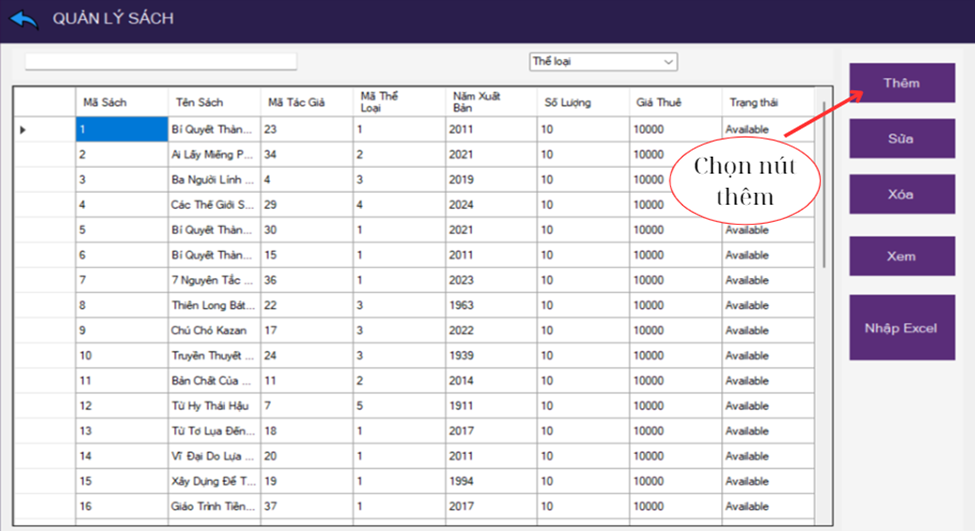
\includegraphics[width=0.8\linewidth]{images//Winform/thêm2.png}
    \label{fig:enter-label}
\end{figure}

Bước 3: Nhập thông tin cho sách và nhấn nút Thêm sau khi nhập xong thông tin
\begin{figure} [H]
    \centering
    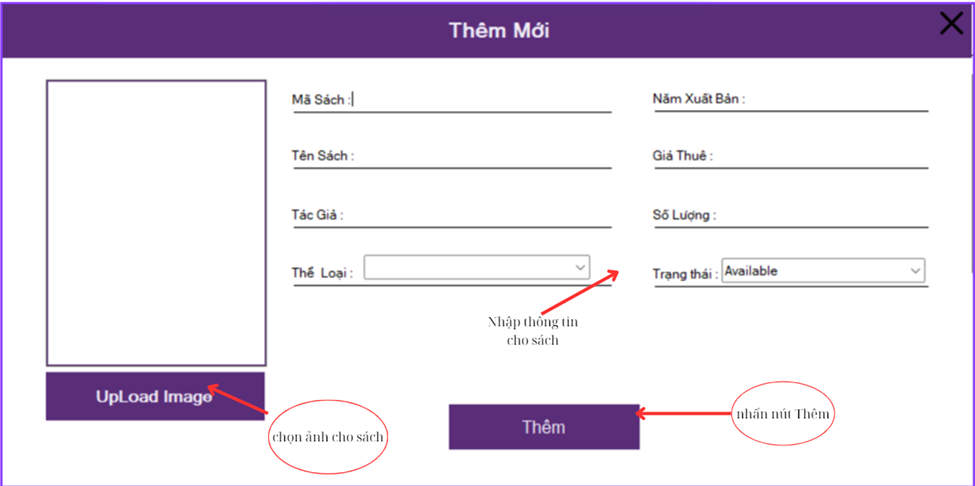
\includegraphics[width=0.8\linewidth]{images//Winform/thêm3.png}
    \label{fig:enter-label}
\end{figure}

Bước 4:Thông báo nếu thêm thành công
\begin{figure} [H]
    \centering
    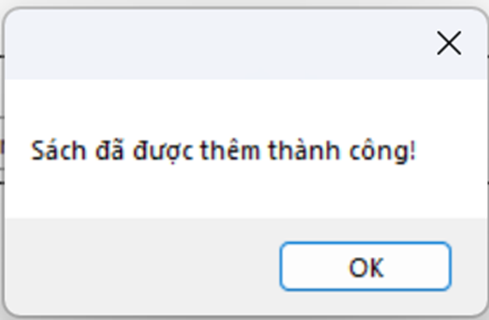
\includegraphics[width=0.5\linewidth]{images/Winform/thêm4.png}
    \label{fig:enter-label}
\end{figure}

\newpage
\subsubsection{Quá trình thực thi sửa sách}
Bước 1: Chọn dữ liệu muốn sửa thông tin
\begin{figure} [H]
    \centering
    \includegraphics[width=0.8\linewidth]{images//Winform/sửa1.png}
    \label{fig:enter-label}
\end{figure}

Bước 2: Chọn nút sửa
\begin{figure} [H]
    \centering
    \includegraphics[width=0.8\linewidth]{images//Winform/sửa2.png}
    \label{fig:enter-label}
\end{figure}

Bước 3:Thực hiện sửa thông tin
\begin{figure} [H]
    \centering
    \includegraphics[width=0.8\linewidth]{images//Winform/sửa3.png}
    \label{fig:enter-label}
\end{figure}

Bước 4: Thông báo 
\begin{figure} [H]
    \centering
    \includegraphics[width=0.5\linewidth]{images/Winform/sửa4.png}
    \label{fig:enter-label}
\end{figure}

\subsubsection{Quá trình thực thi xóa sách}
Bước 1: Chọn dữ liệu muốn xóa
\begin{figure} [H]
    \centering
    \includegraphics[width=0.8\linewidth]{images//Winform/xóa1.png}
    \label{fig:enter-label}
\end{figure}

Bước 2: Chọn nút xóa
\begin{figure} [H]
    \centering
    \includegraphics[width=0.8\linewidth]{images//Winform/xóa2.png}
    \label{fig:enter-label}
\end{figure}

Bước 3: Xác nhận có xóa sách không
\begin{figure} [H]
    \centering
    \includegraphics[width=0.5\linewidth]{images//Winform/xóa3.png}
    \label{fig:enter-label}
\end{figure}

Bước 4: Thông báo khi xác nhận xóa sách
\begin{figure} [H]
    \centering
    \includegraphics[width=0.5\linewidth]{images//Winform/xóa4.png}
    \label{fig:enter-label}
\end{figure}

\subsection{Chức năng quản lý tác giả}
\begin{figure} [H]
    \centering
    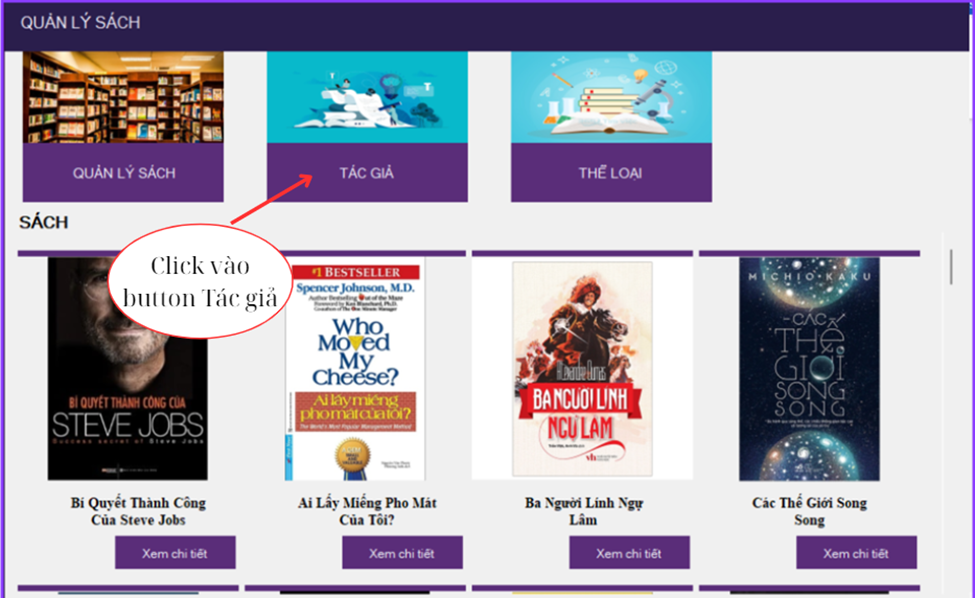
\includegraphics[width=0.8\linewidth]{images//Winform/tác giả.png}
    \label{fig:enter-label}
\end{figure}

\newpage
\subsubsection{Thêm thông tin tác giả}
Bước 1: Nhấn nút Tạo mới
\begin{figure} [H]
    \centering
    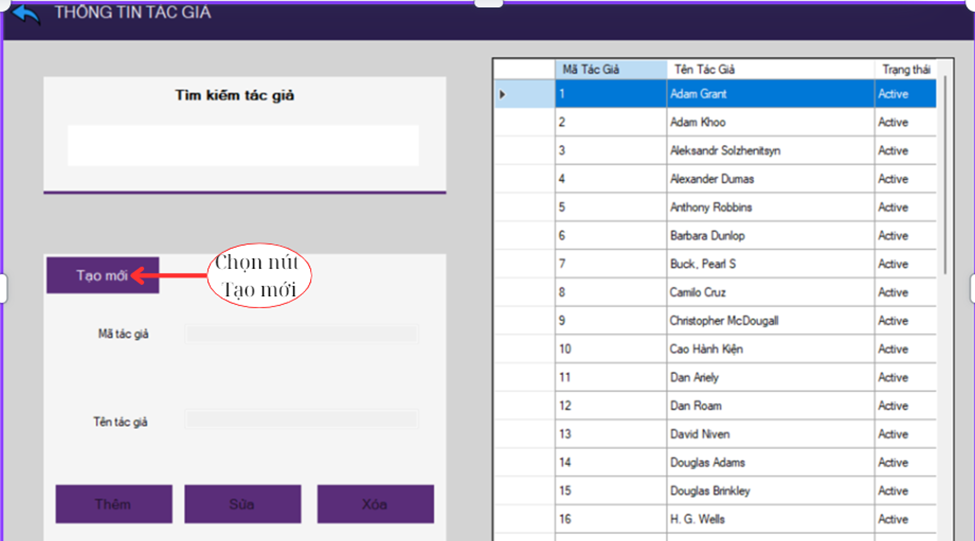
\includegraphics[width=0.8\linewidth]{images//Winform/thêm tg1.png}
    \label{fig:enter-label}
\end{figure}

Bước 2: Nhập tên tác giả và nhấn nút Thêm
\begin{figure} [H]
    \centering
    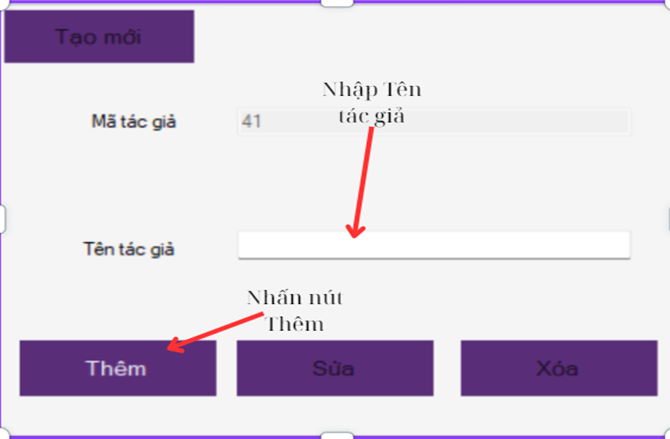
\includegraphics[width=0.5\linewidth]{images//Winform/thêm tg2.png}
    \label{fig:enter-label}
\end{figure}

Bước 3: Thông báo khi thêm thành công
\begin{figure} [H]
    \centering
    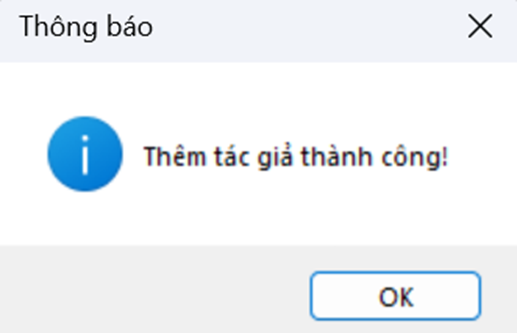
\includegraphics[width=0.5\linewidth]{images/Winform/thêm tg3.png}
    \label{fig:enter-label}
\end{figure}

\newpage
\subsubsection{Sửa thông tin tác giả}
Bước 1: Chọn dữ liệu muốn sửa và nhấn nút sửa
\begin{figure} [H]
    \centering
    \includegraphics[width=0.8\linewidth]{images//Winform/sửa tg1.png}
    \label{fig:enter-label}
\end{figure}

Bước 2: Sửa thông tin và nhấn nút cập nhật
\begin{figure} [H]
    \centering
    \includegraphics[width=0.5\linewidth]{images//Winform/sửa tg2.png}
    \label{fig:enter-label}
\end{figure}

Bước 3: Thông báo
\begin{figure} [H]
    \centering
    \includegraphics[width=0.5\linewidth]{images//Winform/sửa tg3.png}
    \label{fig:enter-label}
\end{figure}

\newpage
\subsubsection{Xóa thông tin tác giả}
Bước 1: Chọn tác giả muốn xóa và nhấn nút xóa
\begin{figure} [H]
    \centering
    \includegraphics[width=0.5\linewidth]{images//Winform/xóa tg1.png}
    \label{fig:enter-label}
\end{figure}

Bước 2: Xác nhận xóa tác giả
\begin{figure} [H]
    \centering
    \includegraphics[width=0.5\linewidth]{images//Winform/xóa tg2.png}
    \label{fig:enter-label}
\end{figure}

Bước 3: Thông báo
\begin{figure} [H]
    \centering
    \includegraphics[width=0.5\linewidth]{images//Winform/xóa tg3.png}
    \label{fig:enter-label}
\end{figure}

\newpage
\subsection{Chức năng quản lý thiết bị}
Tương tự như sách, người dùng có thể thêm, sửa, xóa thiết bị, cập nhật trạng thái, theo dõi số lượng và kiểm tra tình trạng tồn kho thiết bị.

\begin{figure} [H]
    \centering
    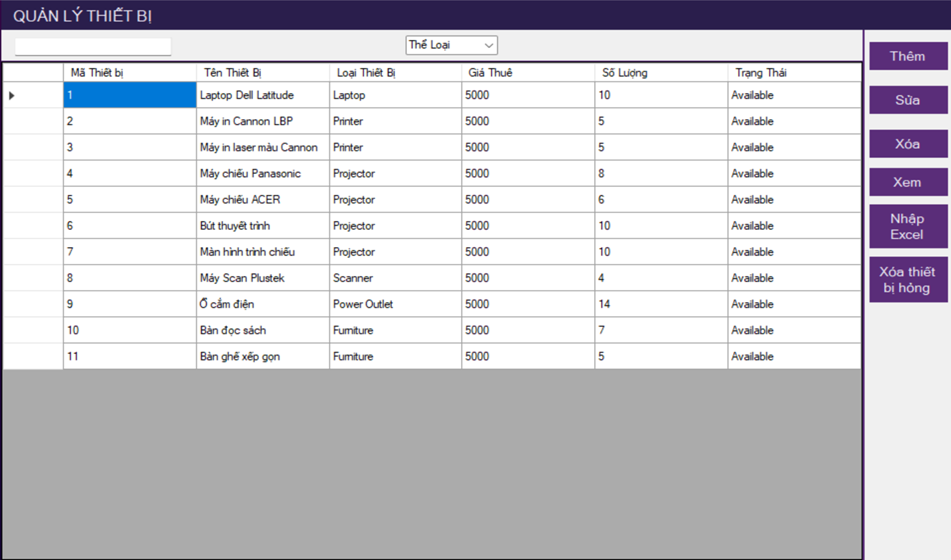
\includegraphics[width=0.8\linewidth]{images//Winform/cn ql tb1.png}
    \caption{Danh sách thiết bị}
    \label{fig:enter-label}
\end{figure}

\begin{figure} [H]
    \centering
    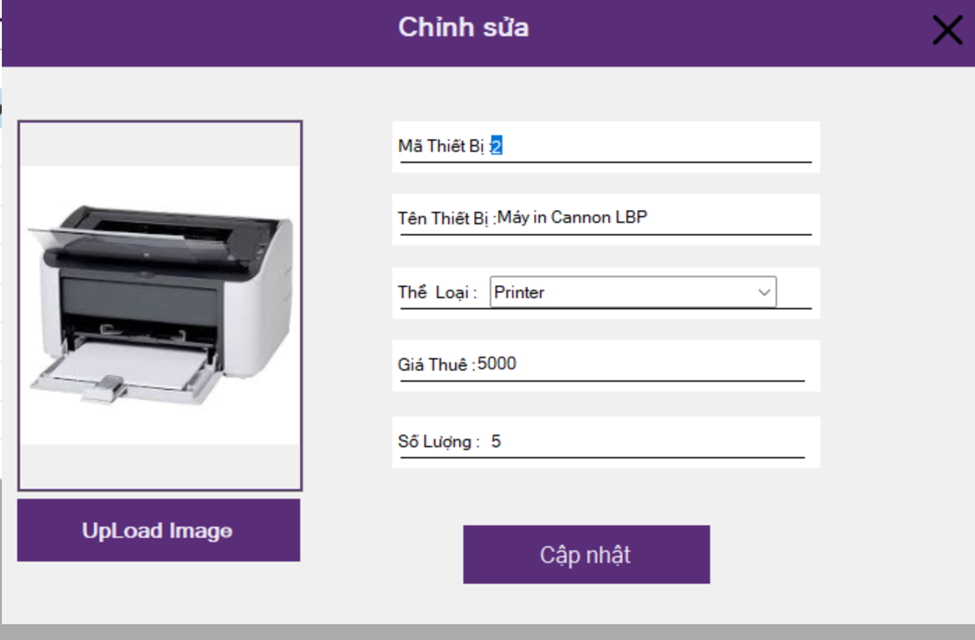
\includegraphics[width=0.8\linewidth]{images//Winform/cn ql tb2.png}
    \caption{Giao diện cập nhật thiết bị}
    \label{fig:enter-label}
\end{figure}

\begin{figure} [H]
    \centering
    \includegraphics[width=0.8\linewidth]{images//Winform/cn ql tb3.png}
    \caption{Giao diện thêm thiết bị}
    \label{fig:enter-label}
\end{figure}

\subsection{Chức năng quản lý thành viên}
Quản lý thông tin người dùng (tên, mã, số điện thoại), tìm kiếm nhanh, phân quyền người dùng (Admin, Nhân viên). Hỗ trợ xóa thành viên không còn hoạt động.

\begin{figure} [H]
    \centering
    \includegraphics[width=0.8\linewidth]{images//Winform/cn ql tv1.png}
    \caption{Giao diện danh sách thành viên}
    \label{fig:enter-label}
\end{figure}

\begin{figure} [H]
    \centering
    \includegraphics[width=0.8\linewidth]{images//Winform/cn ql tv2.png}
    \caption{Thêm thành viên}
    \label{fig:enter-label}
\end{figure}

\begin{figure} [H]
    \centering
    \includegraphics[width=0.8\linewidth]{images//Winform/cn ql tv3.png}
    \caption{Cập nhật thành viên}
    \label{fig:enter-label}
\end{figure}

\newpage
\subsection{Chức năng quản lý giao dịch mượn - trả}
Cho phép tạo giao dịch mượn mới, tự động tính hạn trả, kiểm tra số lượng tồn kho. Khi trả sách hoặc thiết bị, hệ thống cập nhật lại số lượng, tính phí nếu trả trễ và hiển thị thông tin vi phạm nếu có.

\begin{figure} [H]
    \centering
    \includegraphics[width=0.8\linewidth]{images//Winform/cn ql gd1.png}
    \caption{Giao diện đăng ký giao dịch}
    \label{fig:enter-label}
\end{figure}

\begin{figure} [H]
    \centering
    \includegraphics[width=0.8\linewidth]{images//Winform/cn ql gd2.png}
    \caption{Chi tiết thông tin trả}
    \label{fig:enter-label}
\end{figure}

\subsection{Chức năng xử lý vi phậm và thanh toán}
Người dùng có thể thêm vi phạm để xử lý hành vi của thành viên và thực hiện các biện pháp xử lý vi phạm.

\begin{figure} [H]
    \centering
    \includegraphics[width=0.8\linewidth]{images//Winform/cn ql vp1.png}
    \caption{Giao diện quản lý vi phạm}
    \label{fig:enter-label}
\end{figure}

\subsection{Chức năng báo cáo và thống kê}
Thống kê tổng hợp các chỉ số như: số lượt mượn/trả, số lượng sách/thiết bị ,số lượng thành viên vào thư quán và các chức năng lọc theo thời gian ,điều kiện để có được số liệu ưng ý.

\begin{figure} [H]
    \centering
    \includegraphics[width=0.8\linewidth]{images//Winform/cn ql tk1.png}
    \caption{Thống kê số lượng mượn sách}
    \label{fig:enter-label}
\end{figure}

\begin{figure} [H]
    \centering
    \includegraphics[width=0.8\linewidth]{images//Winform/cn ql tk2.png}
    \caption{Thống kê số lượng mượn thiết bị}
    \label{fig:enter-label}
\end{figure}

\begin{figure} [H]
    \centering
    \includegraphics[width=0.8\linewidth]{images//Winform/cn ql tk3.png}
    \caption{Thống kê số lượng mượn thành viên ra vào thư viện}
    \label{fig:enter-label}
\end{figure}


\newpage
\section{Website}
\subsection{Đăng nhập}
Nếu đã có tài khoản thì thực hiện bước nhập tài khoản và mật khẩu vô form.
\begin{figure} [H]
    \centering
    \includegraphics[width=0.4\linewidth]{images//Website/đăng nhập1.png}
    \label{fig:enter-label}
\end{figure}

Nếu như chưa có tài khoản thì thực hiện nhấn nút Đăng ký ngay để chuyển sang form Đăng ký.
\begin{figure} [H]
    \centering
    \includegraphics[width=0.4\linewidth]{images//Website/đăng nhập2.png}
    \label{fig:enter-label}
\end{figure}

\subsection{Thông tin cá nhân}
Thành viên sau khi đăng nhập thành công thì sẽ được chuyển vào trang hồ sơ cá nhân hoặc có thể nhấn nút hồ sơ trên thanh Navbar để chuyển sang trang hồ sơ.
\begin{figure} [H]
    \centering
    \includegraphics[width=1\linewidth]{images//Website/cn ttcn.png}
    \label{fig:enter-label}
\end{figure}

Trong hồ sơ người dùng có thể:
\begin{itemize}
    \item Xem thông tin cá nhân.
    \item Xem những sản phẩm đang mượn và những sản phẩm đặt trước.
    \item Xem lịch sử đã mượn và trả.
    \item Xem số lần vi phạm của thành viên.
    \item Sửa thông tin trong Cài đặt.
\end{itemize}

\subsection{Đặt trước sản phẩm}
\begin{figure} [H]
    \centering
    \includegraphics[width=1\linewidth]{images//Website/cn đặt sách1.png}
    \label{fig:enter-label}
\end{figure}

Ở trang đặt trước sản phẩm thành viên có thể tìm kiếm hoặc lọc sản phẩm để tìm ra sản phẩm mình muốn đặt và nhấn chuột vào nút mượn và thực hiện thiết lập ngày giờ để mà thành viên có thể tới thư quán lấy sản phẩm đã đặt trước.

\begin{figure} [H]
    \centering
    \includegraphics[width=0.5\linewidth]{images//Website/cn đặt sách2.png}
    \label{fig:enter-label}
\end{figure}

\newpage
\bigsection{Tổng kết}
Sau quá trình triển khai và phát triển dự án "Quản Lý Thư Quán", nhóm chúng em đã hoàn thành đầy đủ các chức năng được đặt ra ban đầu cho cả hai nền tảng WinForm và Website, cụ thể:
\begin{itemize}
    \item Về mặt chức năng: Hệ thống hỗ trợ quản lý toàn diện các nghiệp vụ trong thư quán như quản lý sách, thiết bị, thành viên, giao dịch mượn–trả, xử lý vi phạm, thống kê báo cáo và đặt chỗ trực tuyến.
    \item Về mặt kỹ thuật: Dự án ứng dụng mô hình hướng đối tượng (OOP) để thiết kế các lớp dữ liệu rõ ràng, sử dụng cơ sở dữ liệu MySQL kết hợp với giao diện người dùng WinForm cho nghiệp vụ thư viện nội bộ và ASP.NET cho phần giao diện web.
    \item Về giao diện người dùng: Cả hai nền tảng đều được thiết kế trực quan, dễ sử dụng, hướng tới trải nghiệm người dùng và khả năng mở rộng trong tương lai.
    \item Về bảo trì và nâng cấp: Kiến trúc hệ thống phân lớp rõ ràng (Model – DAO – BUS – GUI), dễ dàng chỉnh sửa, mở rộng thêm các chức năng mới hoặc nâng cấp hiệu suất hệ thống.
\end{itemize}

\noindent Hạn chế và hướng phát triển:
\begin{itemize}
    \item Giao diện người dùng, đặc biệt là phần Web, vẫn còn đơn giản, chưa có nhiều yếu tố tương tác nâng cao như chatbot, thông báo thời gian thực, hay tích hợp thanh toán online.
    \item Tính năng phân quyền còn ở mức cơ bản, chủ yếu phân biệt giữa admin và nhân viên, chưa phân chia chi tiết hơn theo từng quyền thao tác cụ thể.
    \item Việc kiểm thử hệ thống chủ yếu thực hiện nội bộ, chưa có điều kiện triển khai thử nghiệm trên quy mô lớn để đánh giá tính ổn định khi có nhiều người dùng đồng thời.
\end{itemize}

\noindent Dựa trên những hạn chế trên, nhóm định hướng nếu có thêm thời gian phát triển sẽ:
\begin{itemize}
    \item Nâng cấp giao diện web theo hướng responsive và tối ưu trải nghiệm người dùng.
    \item Tích hợp thông báo email/SMS khi gần đến hạn trả sách hoặc có vi phạm.
    \item Bổ sung phần quản trị nâng cao với phân quyền chi tiết, kiểm soát log hệ thống và giám sát tài nguyên theo thời gian thực.
    \item Đồng bộ hóa dữ liệu với các chi nhánh thư quán khác nếu triển khai trên quy mô lớn hơn.
\end{itemize}

\noindent Soure code liên quan đến đồ án có thể truy cập tại đây:
\href{https://github.com/ThoiThanhVuong/QuanLyThuQuan}{QuanLyThuQuan}.\\ \\
(https://github.com/ThoiThanhVuong/QuanLyThuQuan)
\end{document}